
\chapter{Introduction}

\begin{definitionblock}[What is Computing?]
    Computing is the process of using computer technology to complete a given goal-oriented task. Computing may encompass the design and development of software and hardware systems for a broad range of purposes. 
\end{definitionblock}

Today, each scientific instrument is critically dependent on computing
for sensor control, data processing, international collaboration,
and access. Computational modelling and data analytics are applicable to all
areas of science and engineering. The ability to use computing
effectively is a key skill for all scientists and engineers.

\begin{figure}[H]
    \centering
    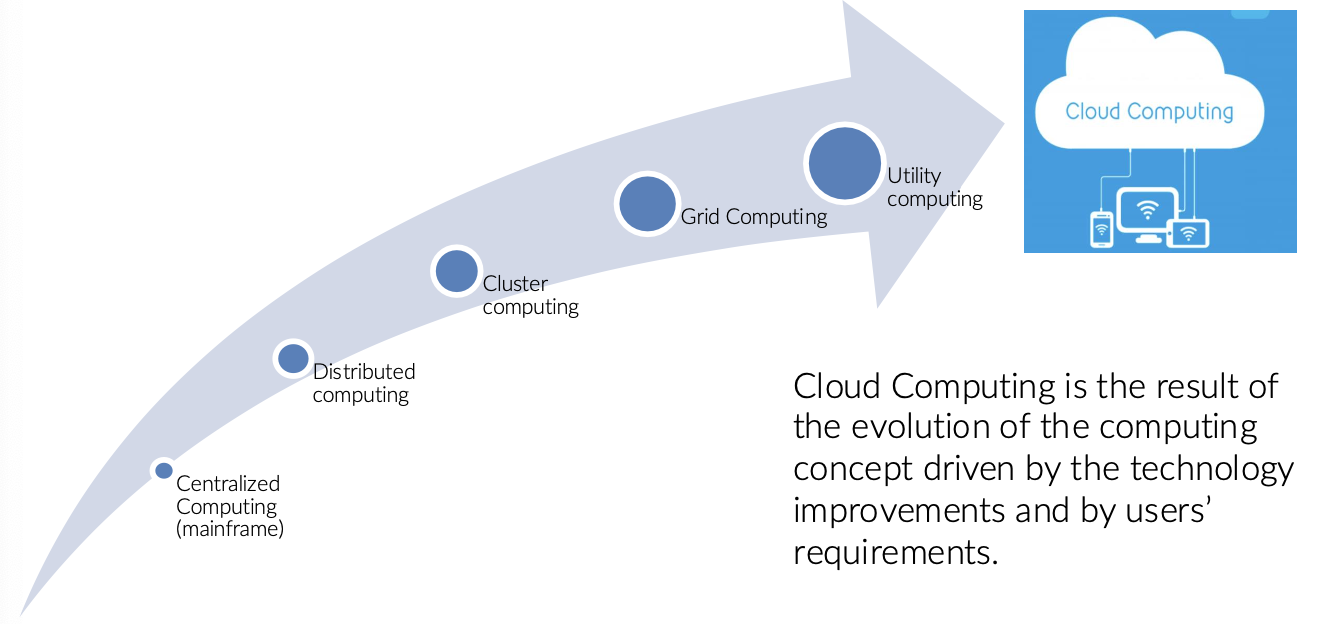
\includegraphics[width=0.8\textwidth]{assets/fig1.png}
    \caption{The evolution of computing.}
    \label{fig:1}
\end{figure}

We can now define what \textbf{Distributed Computing} is:
\begin{definitionblock}[Distributed Computing]
    A distributed system is a collection of autonomous computers that are interconnected with each other and cooperate, thereby sharing resources such as printers and databases.
\end{definitionblock}

A \textbf{DD Architecture} is a distributed system that consists of multiple autonomous computers that communicate through a computer network. The computers interact with each other in order to achieve a common goal. It is based on a client-server model, where the client requests services from the server.

\begin{figure}[H]
    \centering
    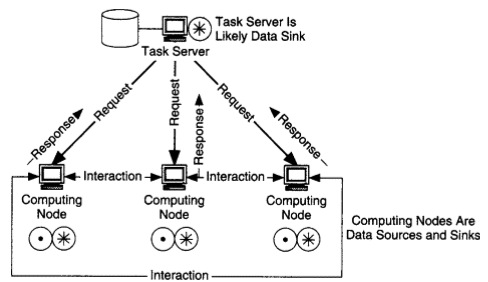
\includegraphics[width=0.5\textwidth]{assets/fig2.png}
    \caption{Distributed Computing.}
    \label{fig:2}
\end{figure}

There is also a 3-tier architecture, where the client interacts with the server, which interacts with the database.

\begin{figure}[H]
    \centering
    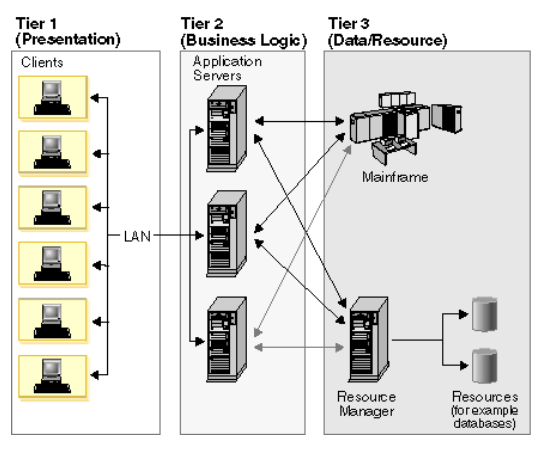
\includegraphics[width=0.5\textwidth]{assets/fig3.png}
    \caption{3-tier architecture.}
    \label{fig:3}
\end{figure}

And finally a peer-to-peer architecture, where each computer can act as a client or a server. Responsibilities are uniformly divided among all machines. 

\begin{figure}[H]
    \centering
    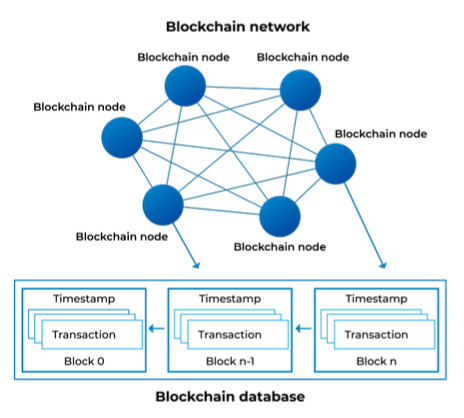
\includegraphics[width=0.4\textwidth]{assets/fig4.png}
    \caption{Peer-to-peer architecture.}
    \label{fig:4}
\end{figure}

\begin{exampleblock}[Hadoop]
    Hadoop is an open-source software framework for storing data and running applications on clusters of commodity hardware. It provides massive storage for any kind of data, enormous processing power and the ability to handle virtually limitless concurrent tasks or jobs.
    It implements a distributed scalable computing model for data analytics, using a \textbf{Distributed File System} (HDFS) and a \textbf{MapReduce} programming model.

    \begin{itemize}
        \item \textbf{HDFS}: Hadoop Distributed File System, a distributed file system that provides high-throughput access to application data. It manages a large number of large files, distributing them across the nodes in a cluster.
        \item \textbf{MapReduce}: a programming model for processing and generating large data sets with a parallel, distributed algorithm on a cluster.
    \end{itemize}
\end{exampleblock}

A \textbf{Computer Cluster} is a group of linked computers, working together closely so that in many respects they form a single computer. The components of a cluster are commonly, but not always, connected to each other through fast local area networks. Clusters are usually deployed to improve performance and availability over that of a single computer, while typically being much more cost-effective than single computers of comparable speed or availability. Clusters are usually deployed to improve performance and/or availability over that provided by a single computer, while typically being much more cost-effective than single computers of comparable speed or availability.
\begin{figure}[H]
    \centering
    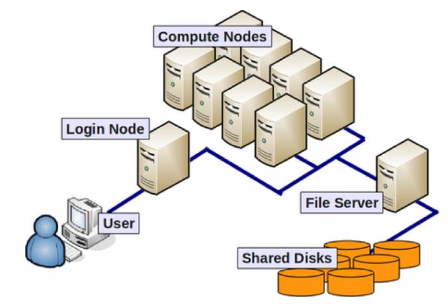
\includegraphics[width=0.5\textwidth]{assets/fig5.png}
    \caption{Computer Cluster.}
    \label{fig:5}
\end{figure}

A cluster can be accessed through a batch system, which is a software system used to manage and schedule batch jobs. Batch systems are used in environments where users do not interactively use a computer system, but instead enter a set of commands to be executed by the system at a later time. The filesystem structure is shared among all nodes in the cluster.

\begin{table}[H]
    \centering
    \begin{tabular}{|p{5cm}|p{5cm}|p{5cm}|} 
    \hline
    \textbf{High Availability Cluster (Linux)} & \textbf{Network Load Balancing Cluster} & \textbf{HPC Cluster} \\ 
    \hline
    Mission-critical applications & Operate by distributing a workload evenly over multiple backend nodes & Low-latency network \\ 
    \hline
    High-availability clusters (aka Failover Clusters) are implemented for the purpose of improving the availability of services which the cluster provides & Typically, the cluster will be configured with multiple redundant load-balancing front ends & Message-passing libraries \\ 
    \hline
    Provide redundancy & All available servers process requests & Parallel filesystem \\ 
    \hline
    Eliminate single points of failure & Web servers, mail servers, etc. & HPC system software \\ 
    \hline
    \end{tabular}
    \caption{Classification of Clusters}
    \label{tab:cluster-classification}
\end{table}

\begin{observationblock}[HPC vs HTC]
    \textbf{High-Performance Computing} (HPC) is the use of parallel processing for running advanced application programs efficiently, reliably and quickly. The term applies especially to systems that function above a teraflop or 10\textsuperscript{12} floating-point operations per second. The term \textbf{High-Throughput Computing} (HTC) refers to the use of many computing resources over long periods of time to accomplish a computational task. 
\end{observationblock}

\begin{itemize}
    \item The \textbf{computing challenge}: In order to to improve the codes’ performance, multi
    (multi–core CPUs) and many cores (GPUs) architectures have to be exploited.
    \item The \textbf{memory challenge}: Huge datasets cannot be loaded in the memory of a
    single CPU and cannot be handled by a single processor but by distributed
    memory systems. Distributed computing, based on the adoption of the MPI
    standard, represents a feasible and effective solution.
    \item \textbf{The data challenge}: This addresses the management, archiving and access of
    the raw data, the science data products, and the final outcomes of data
    processing and analysis.
\end{itemize}
\vspace{0.5cm}
\textbf{N-BODY PROBLEM}
\vspace{0.5cm}

\begin{minipage}{0.48\textwidth}
    The N-body problem broadly
    describes the problem of
    predicting the future
    trajectories of a group of
    objects under the mutual
    gravitational forces they exert
    on one another, given each
    individual object's current
    position and velocity.

    In Astronomy, the N-body
    problem has been studied at a
    wide variety of scales: ranging
    from the study of asteroids
    near Jupiter (Brož et al. 2008)
    to the study of the largest
    gravitationally bound clusters
    in the Universe (Angulo et al.
    2012).
\end{minipage}
\hfill
\begin{minipage}{0.48\textwidth}
    \centering
    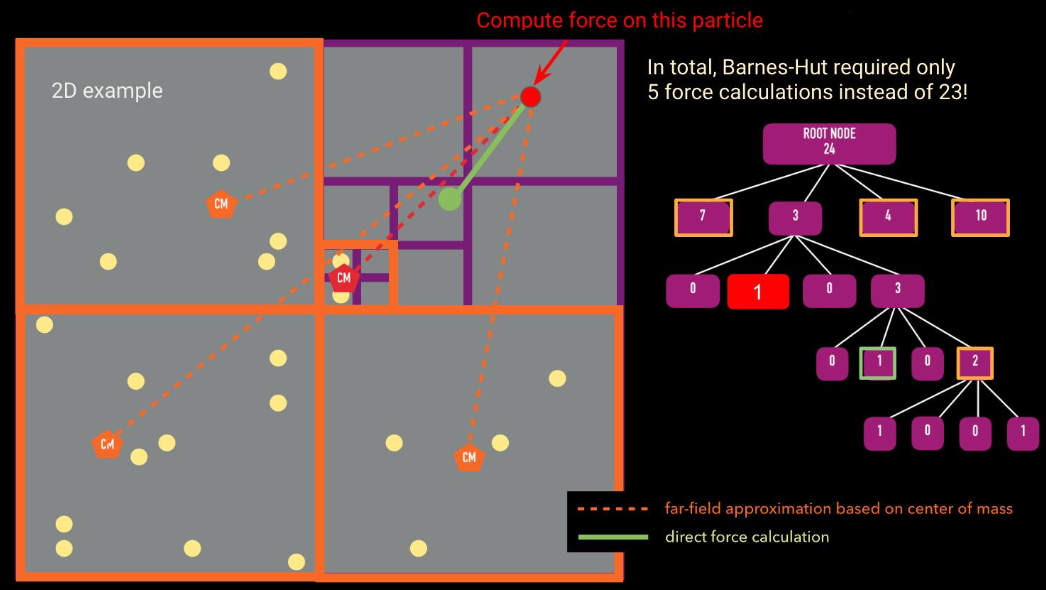
\includegraphics[width=\textwidth]{assets/fig6.png}
\end{minipage}

\newpage 
Including the communication overheads, a simple parallel algorithm has the
following steps:
\begin{enumerate}
    \item Build the Octree (on primary MPI node), Octree is broadcast to all MPI nodes.
    \item For each particle, compute the total force by traversing the Octree (particle positions and velocities are distributed across MPI nodes).
    \item Update the velocities and positions of the particles.
    \item Repeat steps 2 and 3 for a number of time steps.
    \item Output the final positions and velocities of the particles.
\end{enumerate}

\begin{definitionblock}[Grid Computing]
    Grid computing is the collection of computer resources from multiple locations to reach a common goal. The grid can be thought of as a distributed system with non-interactive workloads that involve a large number of files. Grid computing is distinguished from conventional high-performance computing systems such as cluster computing in that grid computers have each node set to perform a different task/application.
\end{definitionblock}

\begin{figure}[H]
    \centering
    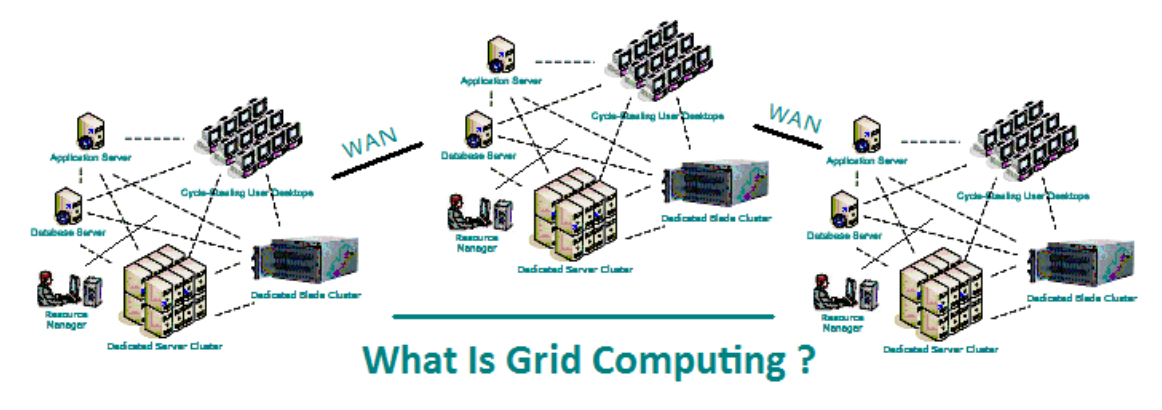
\includegraphics[width=0.8\textwidth]{assets/fig7.png}
    \caption{Grid Computing.}
    \label{fig:7}
\end{figure}

\textbf{Utility computing} is a theoretical concept used in Cloud Computing to provide services based on a metered service model. This model has the advantage of a low or no initial cost to acquire the service; instead, computational resources are essentially rented. The concept is analogous to other utilities, like water and electricity, where the consumer pays for what they use.
\begin{itemize}
    \item Pay-per-use model
    \item Optimize resource utilization
    \item Outsourcing
    \item "Infinite" resources
    \item Access to applications or libraries 
    \item Automation
\end{itemize}

The principle of utility computing is very simple: One company pays
another company for servicing. The services include software rental,
data storage space, use of applications or access to computer processing
power. It all depends on what the client wants and what the company
can offer. Different model may be implemented even if the pay per use is the most
common one (e.g. flat rate, metered, etc). The pricing model is what characterize the Utility Computing.

\begin{figure}[H]
    \centering
    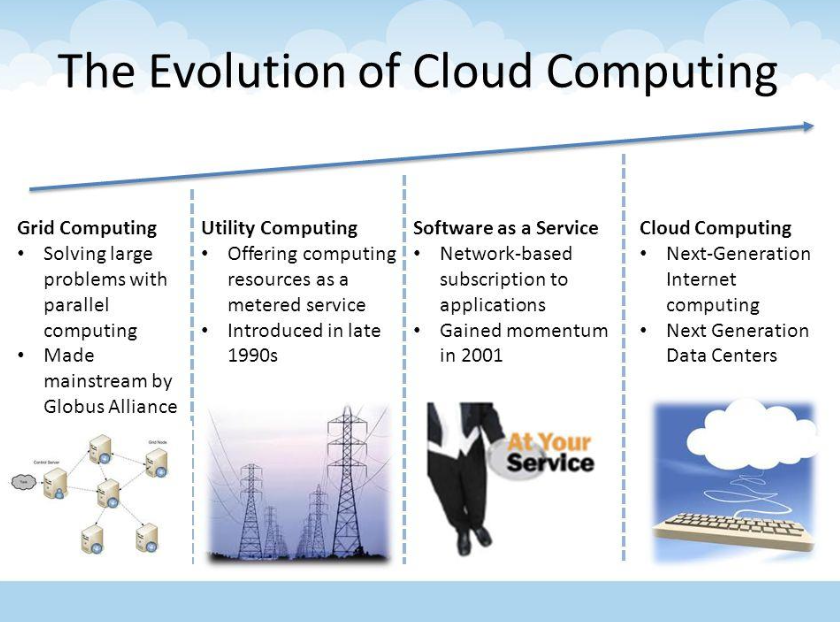
\includegraphics[width=0.8\textwidth]{assets/fig8.png}
\end{figure}

\textbf{Edge Computing} is a distributed
computing paradigm in which
processing and computation are
performed mainly on classified
device nodes known as smart
devices or edge devices as
opposed to processed in a
centralized cloud environment or
data centers. It helps to provide server
resources, data analysis, and
artificial intelligence to data
collection sources and cyber-
physical sources like smart
sensors and actuators.
A network of micro data centers embedded in the
instruments/sensors that store or process critical data
locally and push received data to a centralized data center
or repository of cloud storage. Edge computing processes the data locally results in
reduced traffic in the central repository.

\begin{itemize}
    \item Computing at the edge of the network
    \item Focuses on bringing computing as close to the data source as possible
    \item It decentralizes processing power
    \item It reduces latency
    \item It improves data security
    \item It reduces the amount of data that needs to be moved
    \item It improves scalability
\end{itemize}

\begin{figure}[H]
    \centering
    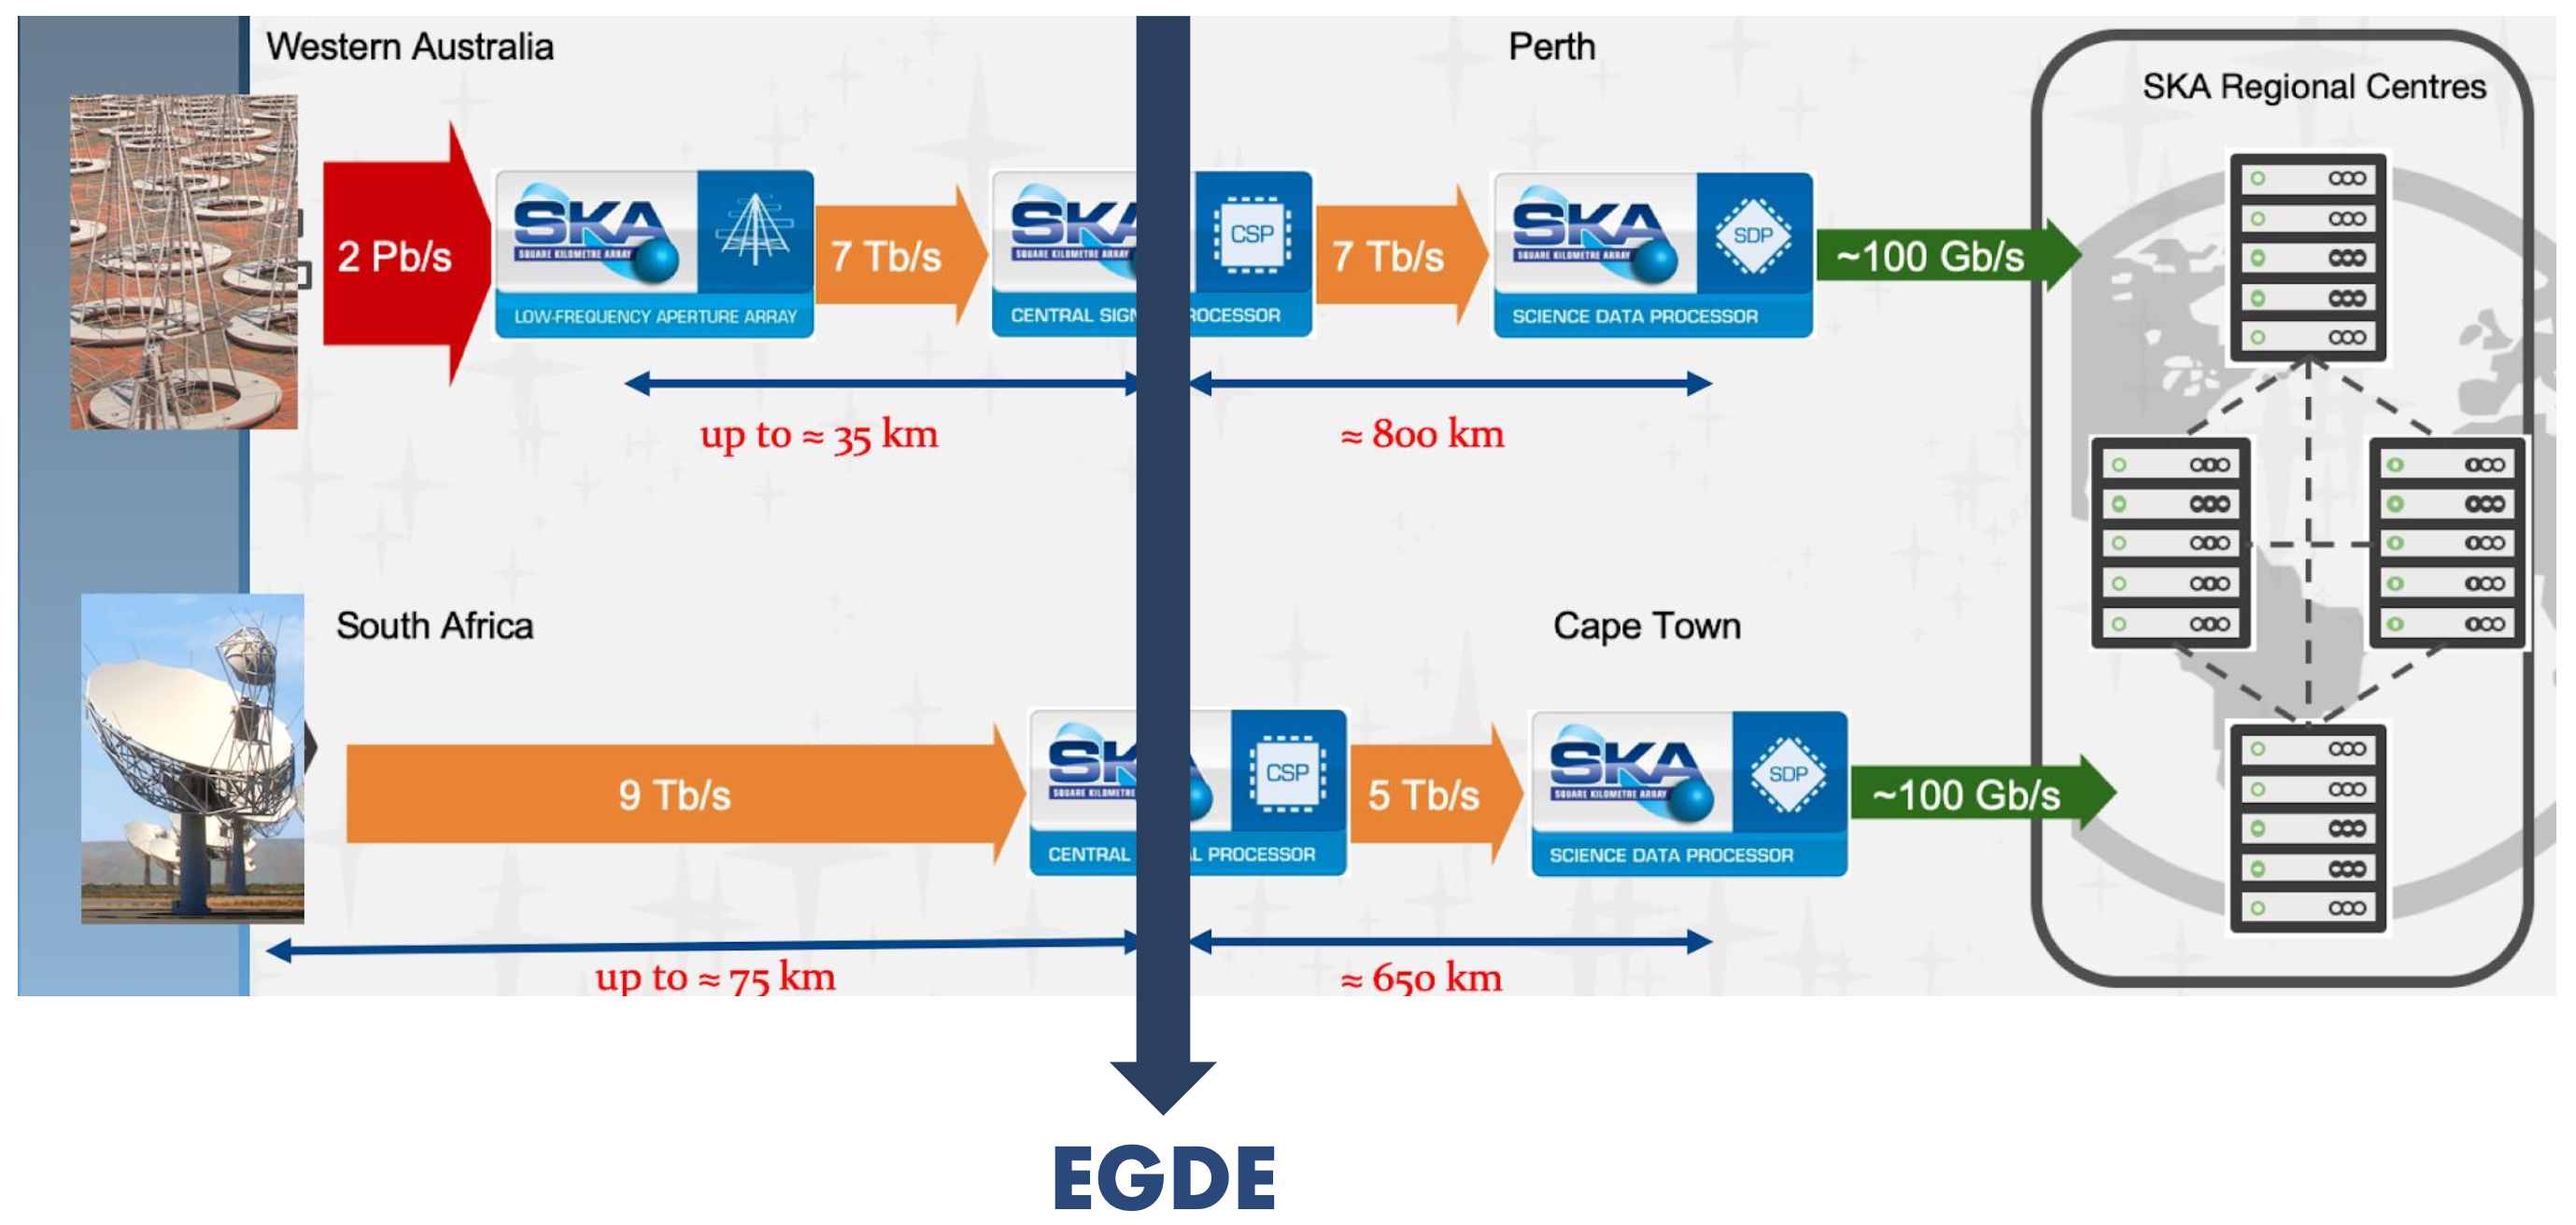
\includegraphics[width=0.6\textwidth]{assets/fig9.png}
    \caption{Edge Computing.}
    \label{fig:9}
\end{figure}








    
